\chapter{Understanding Change Over Time – Change and Motion}

\section{Introduction}
Calculus is the branch of mathematics that focuses on change. While algebra helps us solve for unknown values and geometry deals with shapes and spaces, calculus answers questions about how things change over time, how fast things move, or how quantities accumulate.

Don’t let the idea of calculus intimidate you! At its core, calculus is simply a way of understanding rates of change and accumulation. Whether it’s predicting the speed of a car, calculating areas under curves, or modeling population growth, calculus provides the tools to solve these kinds of problems.

In this chapter, we’ll explore the basics of derivatives and integrals, the two main concepts of calculus, and how they help us describe change and motion.

\section{What Is a Derivative?}
A derivative tells us how a function is changing at any given point. It measures the rate of change or the slope of a curve at a specific point. In simpler terms, it answers questions like:
\begin{itemize}
    \item How fast is a car moving at a specific moment?
    \item How quickly is the population growing?
\end{itemize}

\textbf{Notation:} the following is a table of calculus notations for derivatives and integrals.

\begin{table}[h!]
    \centering
    \begin{tabular}{|l|p{3cm}|p{5cm}|}
        \hline
        \textbf{Notation} & \textbf{Definition} & \textbf{Description} \\
        \hline
        $f'(x)$ & First Derivative of $f(x)$ & Represents the rate of change or slope of $f(x)$ at a point. \\
        \hline
        $\frac{dy}{dx}$ & Derivative of $y$ with respect to $x$ & Common notation for the derivative when $y = f(x)$. \\
        \hline
        $\frac{d}{dx}\left[ f(x) \right]$ & Derivative Operator & Used to denote taking the derivative of $f(x)$ with respect to $x$. \\
        \hline
        $f''(x)$ & Second Derivative of $f(x)$ & Represents the rate of change of $f'(x)$; indicates concavity. \\
        \hline
        $\frac{d^2y}{dx^2}$ & Second Derivative of $y$ with respect to $x$ & Measures how the rate of change itself is changing. \\
        \hline
        $\int f(x) \, dx$ & Indefinite Integral of $f(x)$ & The antiderivative of $f(x)$, representing the area under the curve of $f(x)$. \\
        \hline
        $\int_a^b f(x) \, dx$ & Definite Integral from $a$ to $b$ & Represents the exact area under $f(x)$ from $x = a$ to $x = b$. \\
        \hline
        $\lim_{h \to 0} \frac{f(x+h) - f(x)}{h}$ & Limit Definition of Derivative & Defines the derivative as the limit of the average rate of change. \\
        \hline
        $\partial y / \partial x$ & Partial Derivative of $y$ with respect to $x$ & Used for functions with multiple variables, finding the derivative with respect to one variable while holding others constant. \\
        \hline
    \end{tabular}
    \caption{Common Calculus Notations for Derivatives and Integrals}
\end{table}

\subsection{The Concept of Slope}
In algebra, the slope of a line is a measure of its steepness, and it tells us how fast one variable changes with respect to another. In calculus, the slope is used to describe the instantaneous rate of change of a function.

\subsection{Example}

For a linear function like \( f(x) = 2x + 3 \), the slope is constant. The derivative of this function is 2, meaning the rate of change is the same no matter where you are on the line.

\begin{center}
    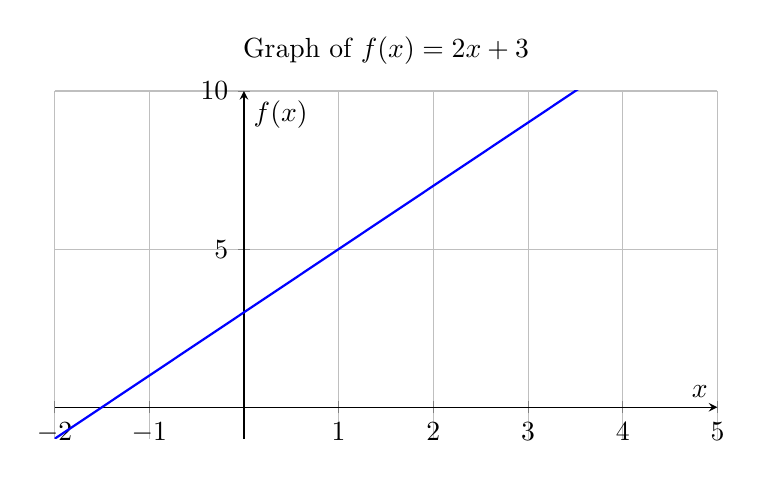
\begin{tikzpicture}
        \begin{axis}[
            axis lines = middle,
            xlabel = \(x\),
            ylabel = {\(f(x)\)},
            ymin=-1, ymax=10,
            xmin=-2, xmax=5,
            grid = major,
            width=10cm,
            height=6cm,
            domain=-2:5,
            samples=100,
            title={Graph of \( f(x) = 2x + 3 \)}
        ]
        \addplot[blue, thick] {2*x + 3};
    \end{axis}
    \end{tikzpicture}
    \captionof{figure}{Graph of the linear function \( f(x) = 2x + 3 \). The slope is constant across the entire line.}
\end{center}

But what happens when the function isn’t a straight line? For functions that curve, like \( f(x) = x^2 \), the slope (or rate of change) varies depending on the point. The derivative helps us figure out the slope at any point along the curve.

\begin{center}
    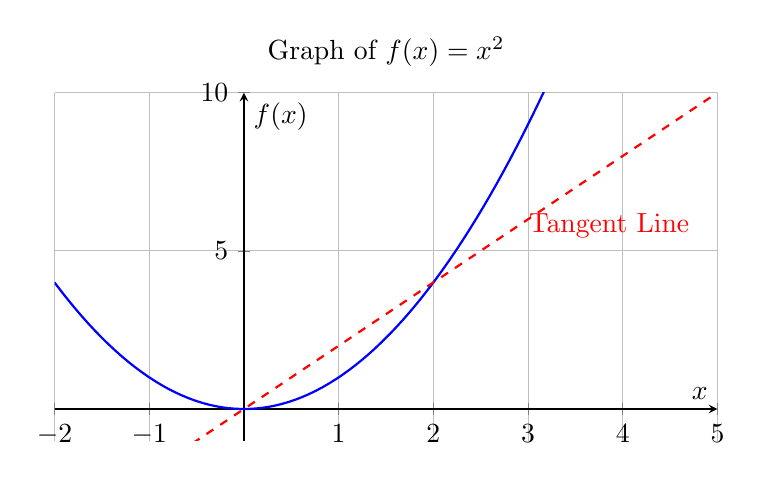
\begin{tikzpicture}
        \begin{axis}[
            axis lines = middle,
            xlabel = \(x\),
            ylabel = {\(f(x)\)},
            ymin=-1, ymax=10,
            xmin=-2, xmax=5,
            grid = major,
            width=10cm,
            height=6cm,
            domain=-2:5,
            samples=100,
            title={Graph of \( f(x) = x^2 \)}
        ]
        \addplot[blue, thick] {x^2};
        \addplot[red, dashed, thick, domain=-2:5] {2*x} node [pos=0.7, right] {Tangent Line};
    \end{axis}
    \end{tikzpicture}
    \captionof{figure}{Graph of the quadratic function \( f(x) = x^2 \). The red dashed line shows a tangent at a point, illustrating the slope at that specific point. The slope of the tangent line represents the derivative of the function at that point, which gives the instantaneous rate of change of the function. As the point moves along the curve, the slope of the tangent line changes, reflecting the varying rate of change of the function. This demonstrates how the derivative provides valuable information about the behavior of the function at different points.}
\end{center}

\section{Finding Derivatives}

The derivative of a function helps us find the rate of change, which can be calculated using specific rules. These rules make it easier to determine how different functions change.

\begin{itemize}
    \item \textbf{Power Rule:} If $f(x) = x^n$, then the derivative is $f'(x) = n \cdot x^{n-1}$.
    
    \begin{center}
        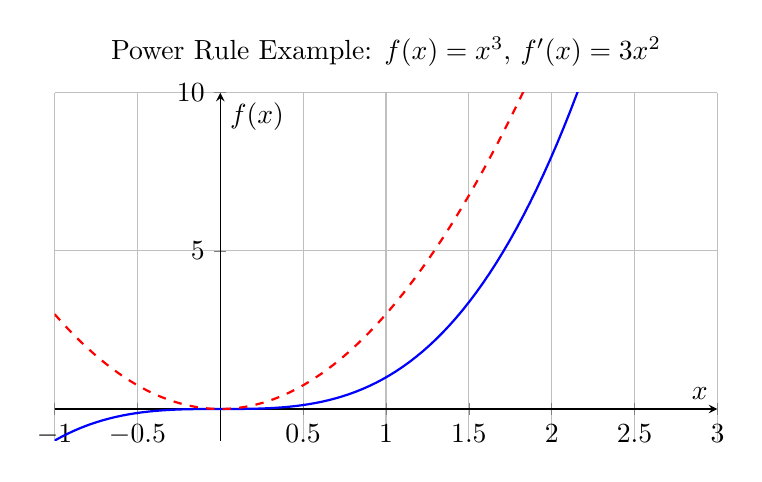
\begin{tikzpicture}
            \begin{axis}[
                axis lines = middle,
                xlabel = $x$,
                ylabel = {$f(x)$},
                ymin=-1, ymax=10,
                xmin=-1, xmax=3,
                grid = major,
                width=10cm,
                height=6cm,
                domain=-1:3,
                samples=100,
                title={Power Rule Example: $f(x) = x^3$, $f'(x) = 3x^2$}
            ]
            \addplot[blue, thick] {x^3};
            \addplot[red, dashed, thick] {3*x^2};
        \end{axis}
        \end{tikzpicture}
        \captionof{figure}{Graph of $f(x) = x^3$ (blue) and its derivative $f'(x) = 3x^2$ (red dashed). The derivative represents the rate of change of the curve.}
    \end{center}

    \item \textbf{Constant Rule:} The derivative of a constant function is zero.
    
    \begin{center}
        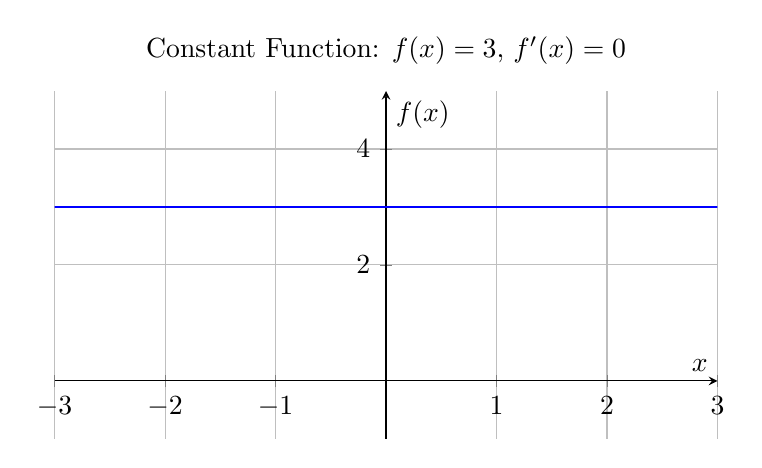
\begin{tikzpicture}
            \begin{axis}[
                axis lines = middle,
                xlabel = $x$,
                ylabel = {$f(x)$},
                ymin=-1, ymax=5,
                xmin=-3, xmax=3,
                grid = major,
                width=10cm,
                height=6cm,
                title={Constant Function: $f(x) = 3$, $f'(x) = 0$}
            ]
            \addplot[blue, thick] {3};
        \end{axis}
        \end{tikzpicture}
        \captionof{figure}{Graph of the constant function $f(x) = 3$. The slope of this function is zero everywhere, hence $f'(x) = 0$.}
    \end{center}

    \item \textbf{Sum Rule:} The derivative of the sum of functions is the sum of their derivatives.
    
    \begin{center}
        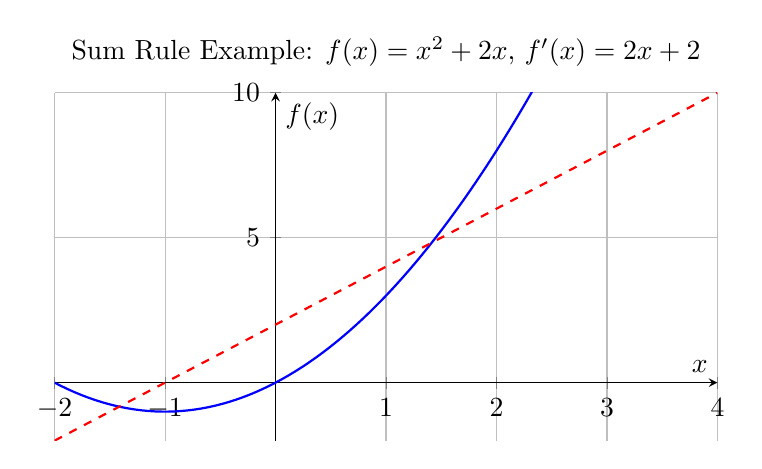
\begin{tikzpicture}
            \begin{axis}[
                axis lines = middle,
                xlabel = $x$,
                ylabel = {$f(x)$},
                ymin=-2, ymax=10,
                xmin=-2, xmax=4,
                grid = major,
                width=10cm,
                height=6cm,
                domain=-2:4,
                samples=100,
                title={Sum Rule Example: $f(x) = x^2 + 2x$, $f'(x) = 2x + 2$}
            ]
            \addplot[blue, thick] {x^2 + 2*x};
            \addplot[red, dashed, thick] {2*x + 2};
        \end{axis}
        \end{tikzpicture}
        \captionof{figure}{Graph of $f(x) = x^2 + 2x$ (blue) and its derivative $f'(x) = 2x + 2$ (red dashed). The derivative is the sum of the derivatives of $x^2$ and $2x$.}
    \end{center}

    \item \textbf{Product Rule:} The derivative of the product of two differentiable functions is given by:
    
    \[ f(x) = g(x) \cdot h(x) \quad \Rightarrow \quad f'(x) = g'(x) \cdot h(x) + g(x) \cdot h'(x) \]
    
    \textbf{Example:} If $f(x) = x^2 \cdot \sin(x)$:
    \begin{enumerate}
        \item Set $g(x) = x^2$ and $h(x) = \sin(x)$.
        \item Compute $g'(x) = 2x$ and $h'(x) = \cos(x)$.
        \item Substitute into the Product Rule:
        \[ f'(x) = (2x) \cdot \sin(x) + x^2 \cdot \cos(x) \]
    \end{enumerate}
    
    \begin{center}
        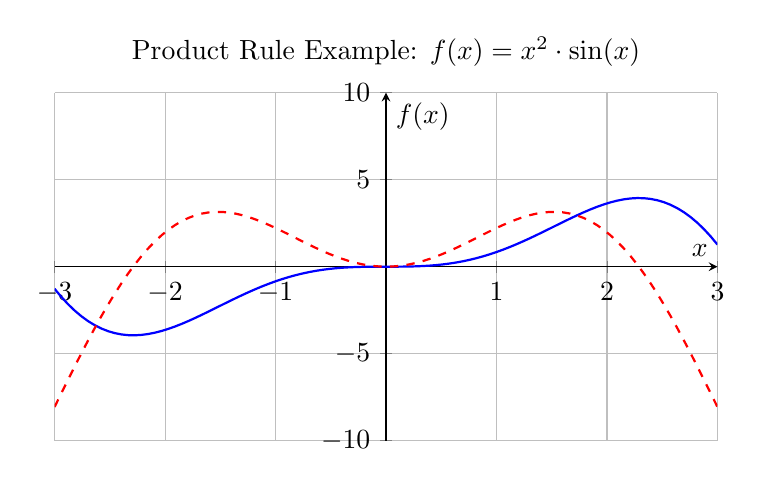
\begin{tikzpicture}
            \begin{axis}[
                axis lines = middle,
                xlabel = $x$,
                ylabel = {$f(x)$},
                ymin=-10, ymax=10,
                xmin=-3, xmax=3,
                grid = major,
                width=10cm,
                height=6cm,
                domain=-3:3,
                samples=100,
                title={Product Rule Example: $f(x) = x^2 \cdot \sin(x)$}
            ]
            \addplot[blue, thick] {x^2 * sin(deg(x))};
            \addplot[red, dashed, thick] {2*x*sin(deg(x)) + x^2*cos(deg(x))};
        \end{axis}
        \end{tikzpicture}
        \captionof{figure}{Graph of $f(x) = x^2 \cdot \sin(x)$ (blue) and its derivative $f'(x)$ (red dashed).}
    \end{center}

    \begin{center}
        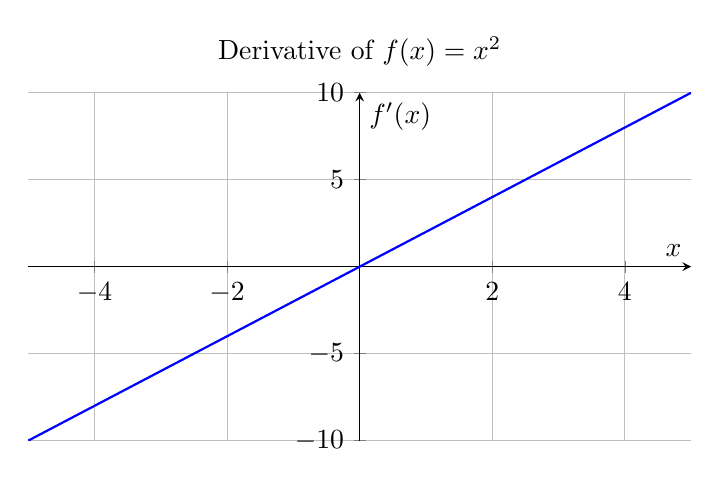
\begin{tikzpicture}
            \begin{axis}[
                axis lines = middle,
                xlabel = $x$,
                ylabel = {$f'(x)$},
                ymin=-10, ymax=10,
                xmin=-5, xmax=5,
                grid = major,
                width=10cm,
                height=6cm,
                domain=-5:5,
                samples=100,
                title={Derivative of $f(x) = x^2$}
                ]
            \addplot[blue, thick] {2*x};
            \end{axis}
        \end{tikzpicture}
        \captionof{figure}{Graph of the derivative $f'(x) = 2x$ of the function $f(x) = x^2$. The slope of $f(x)$ changes depending on the value of $x$.}
    \end{center}
\end{itemize}


\subsection{Basic Rules for Derivatives}
\begin{enumerate}
    \item \textbf{Power Rule:} For any function of the form $f(x) = x^n$, where $n$ is a constant, the derivative is:
    \[ f'(x) = n \cdot x^{n-1} \]
    \textbf{Examples:}
    \begin{itemize}
        \item For $f(x) = x^2$, the derivative is: $f'(x) = 2x$
        \item For $f(x) = x^3$, the derivative is: $f'(x) = 3x^2$
    \end{itemize}
    
    \item \textbf{Constant Rule:} The derivative of a constant is always 0. This is because a constant does not change, so its rate of change is 0.
    \textbf{Example:}
    \begin{itemize}
        \item For $f(x) = 7$, the derivative is $f'(x) = 0$.
    \end{itemize}
    
    \item \textbf{Sum and Difference Rule:} If you have two functions being added or subtracted, you can find the derivative of each part separately.
    \textbf{Example:}
    \begin{itemize}
        \item For $f(x) = 3x^2 + 4x$, the derivative is: $f'(x) = 6x + 4$
    \end{itemize}
\end{enumerate}

\subsection{Interpreting Derivatives}
The derivative gives you the slope of a curve at any point. If the slope is positive, the function is increasing at that point; if the slope is negative, the function is decreasing.

\section{Applications of Derivatives}
Derivatives are incredibly useful in real-world scenarios. Let’s look at a few practical examples:
\begin{enumerate}
    \item \textbf{Velocity:} If you know the position of an object as a function of time, the derivative of that function gives you the object’s velocity, or the rate of change of position.

    \textbf{Example:} Suppose the position of a car over time is given by \( f(t) = t^2 \).
    \begin{itemize}
        \item The derivative, \( f'(t) = 2t \), tells us the car’s velocity at any time \( t \).
    \end{itemize}
    
    \begin{center}
        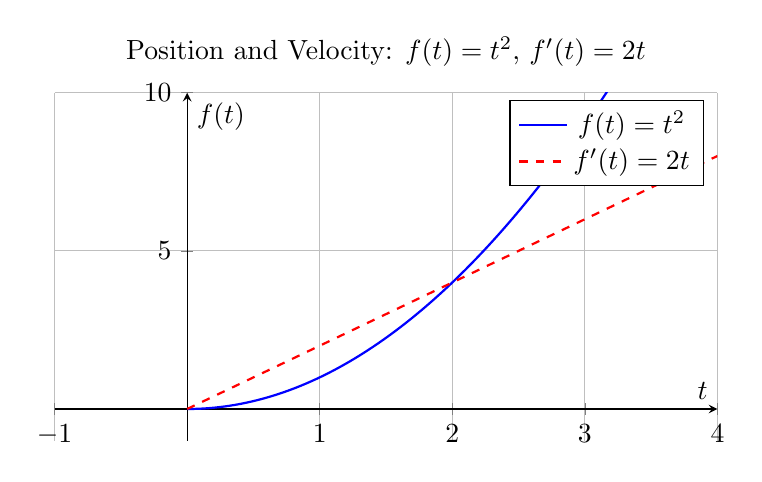
\begin{tikzpicture}
            \begin{axis}[
                axis lines = middle,
                xlabel = $t$,
                ylabel = {$f(t)$},
                ymin=-1, ymax=10,
                xmin=-1, xmax=4,
                grid = major,
                width=10cm,
                height=6cm,
                domain=0:4,
                samples=100,
                title={Position and Velocity: $f(t) = t^2$, $f'(t) = 2t$}
            ]
            \addplot[blue, thick] {x^2};
            \addplot[red, dashed, thick] {2*x};
            \legend{$f(t) = t^2$, $f'(t) = 2t$}
        \end{axis}
        \end{tikzpicture}
        \captionof{figure}{Graph of position \( f(t) = t^2 \) (blue) and its velocity \( f'(t) = 2t \) (red dashed). The slope of the position function represents the car's velocity over time.}
    \end{center}

    \item \textbf{Optimization:} Businesses use derivatives to find maximum profits or minimum costs. By taking the derivative of a profit or cost function, companies can determine when profits are at their highest or when costs are at their lowest.

    \textbf{Example:} Suppose the profit function of a business is \( P(x) = -2x^2 + 12x + 5 \), where \( x \) is the number of items produced and sold.
    \begin{itemize}
        \item To maximize profit, we first need to find the critical points of the profit function. Critical points occur where the derivative is zero or undefined, as these points can indicate potential maximum or minimum values.
    
        \item Given the profit function \( P(x) = -2x^2 + 12x + 5 \), we start by finding its first derivative, \( P'(x) \), which gives us the rate of change of profit with respect to the quantity \( x \):
        \[
        P(x) = -2x^2 + 12x + 5
        \]
        \[
        P'(x) = \frac{d}{dx}(-2x^2 + 12x + 5) = -4x + 12
        \]
    
        \item To find the critical points, we set \( P'(x) \) equal to zero and solve for \( x \):
        \[
        -4x + 12 = 0
        \]
        \[
        -4x = -12
        \]
        \[
        x = 3
        \]
        
        \item We now have a critical point at \( x = 3 \). To confirm whether this point is a maximum, we can examine the second derivative \( P''(x) \):
        
        \item Calculating the second derivative:
        \[
        P''(x) = \frac{d}{dx}(-4x + 12) = -4
        \]
        Since \( P''(x) = -4 < 0 \), the second derivative is negative, indicating that the graph of \( P(x) \) is concave down at \( x = 3 \). Therefore, \( x = 3 \) is indeed a maximum point.
    
        \item Thus, at \( x = 3 \), the business achieves maximum profit. To find the maximum profit value, we substitute \( x = 3 \) back into the original profit function:
        \[
        P(3) = -2(3)^2 + 12 \cdot 3 + 5
        \]
        \[
        = -2 \cdot 9 + 36 + 5
        \]
        \[
        = -18 + 36 + 5 = 23
        \]
    
        \item Therefore, the maximum profit the business can achieve is \( P(3) = 23 \) when \( x = 3 \).
    \end{itemize}
    

    \begin{center}
        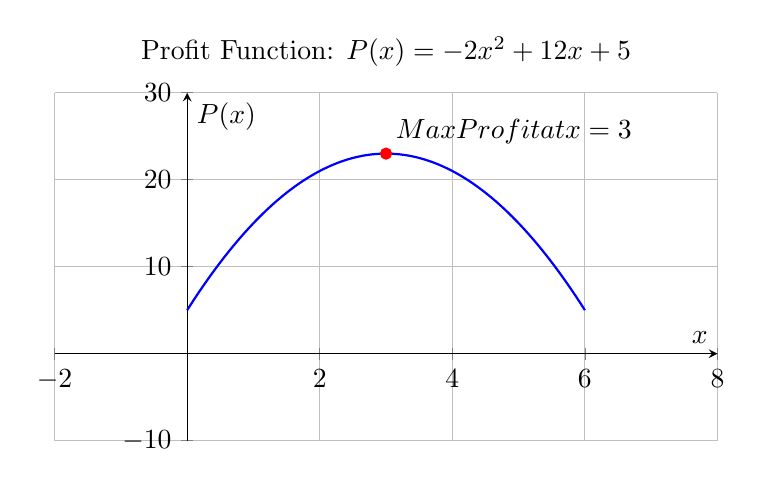
\begin{tikzpicture}
            \begin{axis}[
                axis lines = middle,
                xlabel = $x$,
                ylabel = {$P(x)$},
                ymin=-10, ymax=30,
                xmin=-2, xmax=8,
                grid = major,
                width=10cm,
                height=6cm,
                domain=0:6,
                samples=100,
                title={Profit Function: $P(x) = -2x^2 + 12x + 5$}
            ]
            \addplot[blue, thick] {-2*x^2 + 12*x + 5};
            \addplot[red, mark=*] coordinates {(3,23)};
            \node at (axis cs:3,23) [above right] {$\text{Max Profit at } x=3$};
        \end{axis}
        \end{tikzpicture}
        \captionof{figure}{Graph of the profit function \( P(x) = -2x^2 + 12x + 5 \) with a maximum at \( x = 3 \).}
    \end{center}

    \item \textbf{Tangent Lines:} The derivative of a function at a point gives the slope of the tangent line to the curve at that point. A tangent line is a straight line that touches the curve at exactly one point and represents the best linear approximation of the curve near that point.

    \textbf{Example:} Let \( f(x) = x^2 \). To find the tangent line at \( x = 1 \):
    \begin{itemize}
        \item We start with the function \( f(x) = x^2 \), and we want to find the equation of the tangent line to this function at the point \( x = 1 \).
    
        \item To find the slope of the tangent line, we compute the derivative of \( f(x) \), which gives us the rate of change of \( f(x) \) at any point \( x \):
        \[
        f(x) = x^2
        \]
        \[
        f'(x) = \frac{d}{dx}(x^2) = 2x
        \]
    
        \item Now, we evaluate the derivative at \( x = 1 \) to find the slope of the tangent line at this point:
        \[
        f'(1) = 2 \cdot 1 = 2
        \]
        Thus, the slope of the tangent line at \( x = 1 \) is \( 2 \).
    
        \item Next, we need the coordinates of the point on the curve at \( x = 1 \) to write the tangent line's equation. We substitute \( x = 1 \) into the original function \( f(x) = x^2 \) to find \( f(1) \):
        \[
        f(1) = (1)^2 = 1
        \]
        So, the point of tangency on the curve is \( (1, 1) \).
    
        \item With the point \( (1, 1) \) and the slope \( 2 \), we can now write the equation of the tangent line. The equation of a line with slope \( m \) passing through a point \( (x_0, y_0) \) is given by:
        \[
        y = y_0 + m(x - x_0)
        \]
        Substituting \( x_0 = 1 \), \( y_0 = 1 \), and \( m = 2 \), we get:
        \[
        y = 1 + 2(x - 1)
        \]
    
        \item Expanding and simplifying this expression, we find:
        \[
        y = 1 + 2x - 2 = 2x - 1
        \]
        
        \item Therefore, the equation of the tangent line to the curve \( f(x) = x^2 \) at the point \( x = 1 \) is:
        \[
        y = 2x - 1
        \]
    \end{itemize}
    

    \begin{center}
        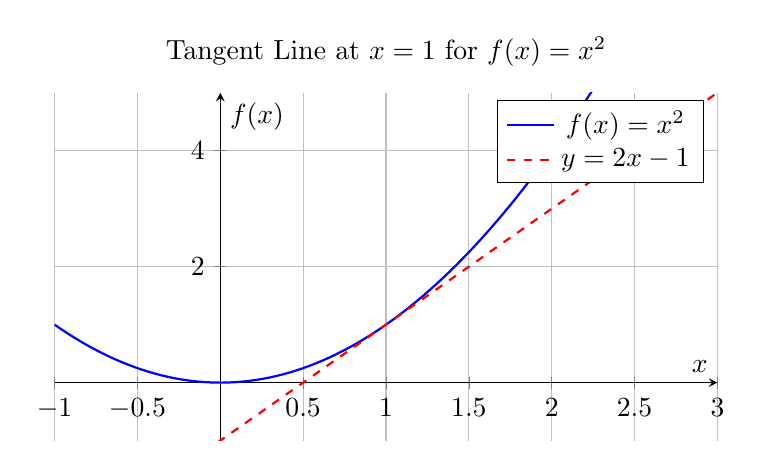
\begin{tikzpicture}
            \begin{axis}[
                axis lines = middle,
                xlabel = $x$,
                ylabel = {$f(x)$},
                ymin=-1, ymax=5,
                xmin=-1, xmax=3,
                grid = major,
                width=10cm,
                height=6cm,
                domain=-1:3,
                samples=100,
                title={Tangent Line at $x = 1$ for $f(x) = x^2$}
            ]
            \addplot[blue, thick] {x^2};
            \addplot[red, dashed, thick] {2*x - 1};
            \legend{$f(x) = x^2$, $y = 2x - 1$}
        \end{axis}
        \end{tikzpicture}
        \captionof{figure}{Graph of \( f(x) = x^2 \) (blue) and its tangent line at \( x = 1 \), \( y = 2x - 1 \) (red dashed). The tangent line touches the curve at exactly one point, providing a linear approximation.}
    \end{center}
\end{enumerate}


\section{What Is an Integral?}
While derivatives focus on how things change, integrals help us calculate how much has accumulated over time. An integral measures the area under a curve.

Imagine you’re tracking the speed of a car over time. The integral of the speed function gives you the total distance the car has traveled.

\subsection{The Concept of Area}
In algebra, you can find the area of simple shapes like rectangles and triangles. In calculus, integrals allow you to find the area under curves, even if the shape is irregular.

\section{Finding Integrals}
Just like derivatives, there are rules for finding integrals. These rules help you calculate the total accumulation or area under a curve.

\subsection{Basic Rules for Integrals}
\begin{enumerate}
    \item \textbf{Power Rule for Integrals:} For any function of the form \( f(x) = x^n \), where \( n \neq -1 \), the power rule for integrals allows us to integrate by increasing the exponent by 1 and dividing by the new exponent. Mathematically, this is expressed as:
    \[
    \int x^n \, dx = \frac{x^{n+1}}{n+1} + C
    \]
    where \( C \) is the constant of integration, representing an arbitrary constant since indefinite integrals have multiple solutions.

    \textbf{Explanation:} To find the antiderivative of \( x^n \), we observe that differentiating \( \frac{x^{n+1}}{n+1} \) gives \( x^n \) back. This is because applying the reverse of the power rule for derivatives yields the original function, confirming that the integral is correct.

    \textbf{Example:} For \( f(x) = x^2 \), we apply the power rule:
    \[
    \int x^2 \, dx = \frac{x^{2+1}}{2+1} + C = \frac{x^3}{3} + C
    \]
    This integral shows that the antiderivative of \( x^2 \) is \( \frac{x^3}{3} \) plus a constant \( C \), indicating that any function of the form \( \frac{x^3}{3} + C \) would differentiate back to \( x^2 \).

    \begin{center}
        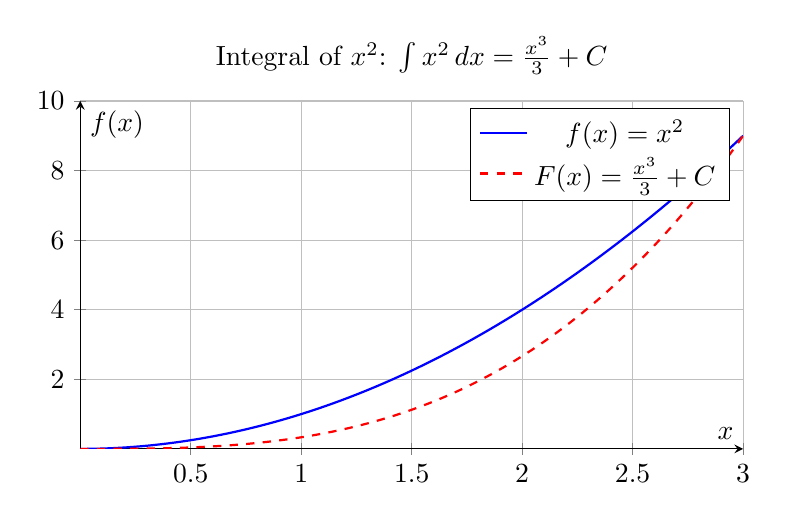
\begin{tikzpicture}
            \begin{axis}[
                axis lines = middle,
                xlabel = $x$,
                ylabel = {$f(x)$},
                ymin=0, ymax=10,
                xmin=0, xmax=3,
                grid = major,
                width=10cm,
                height=6cm,
                domain=0:3,
                samples=100,
                title={Integral of $x^2$: $\int x^2 \, dx = \frac{x^3}{3} + C$}
            ]
            \addplot[blue, thick] {x^2};
            \addplot[red, thick, dashed, domain=0:3] {x^3 / 3};
            \legend{$f(x) = x^2$, $F(x) = \frac{x^3}{3} + C$}
        \end{axis}
        \end{tikzpicture}
        \captionof{figure}{Graph of $f(x) = x^2$ (blue) and its antiderivative $F(x) = \frac{x^3}{3} + C$ (red dashed).}
    \end{center}

    \item \textbf{Constant Rule for Integrals:} The integral of a constant \( a \) is the constant multiplied by \( x \):
    \[
    \int a \, dx = a \cdot x + C
    \]
    where \( C \) is the constant of integration.

    \textbf{Explanation:} Integrating a constant is equivalent to finding a function whose derivative would result in that constant. Since the derivative of \( ax + C \) with respect to \( x \) is \( a \), we see that \( a \cdot x + C \) is indeed the antiderivative of \( a \).

    \textbf{Example:} For \( f(x) = 5 \), we find:
    \[
    \int 5 \, dx = 5x + C
    \]
    This result shows that the antiderivative of a constant function \( 5 \) is \( 5x \) plus an arbitrary constant \( C \), as any constant term would disappear upon differentiation.

    \begin{center}
        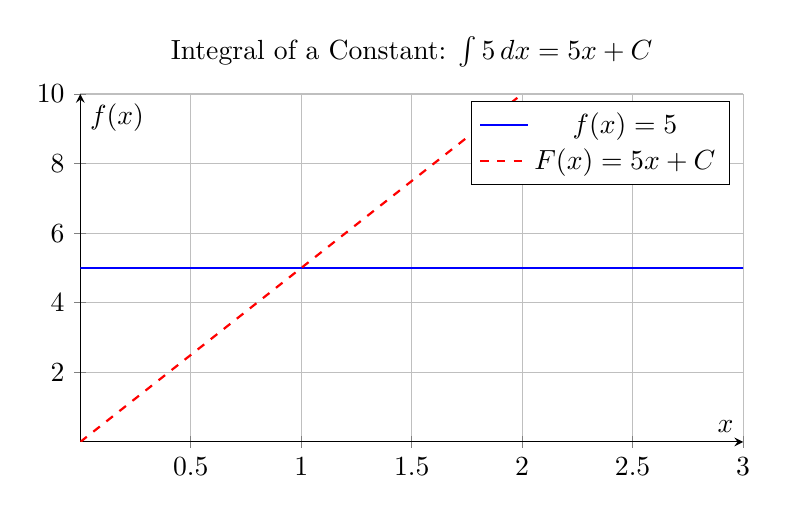
\begin{tikzpicture}
            \begin{axis}[
                axis lines = middle,
                xlabel = $x$,
                ylabel = {$f(x)$},
                ymin=0, ymax=10,
                xmin=0, xmax=3,
                grid = major,
                width=10cm,
                height=6cm,
                title={Integral of a Constant: $\int 5 \, dx = 5x + C$}
            ]
            \addplot[blue, thick] {5};
            \addplot[red, thick, dashed, domain=0:3] {5 * x};
            \legend{$f(x) = 5$, $F(x) = 5x + C$}
        \end{axis}
        \end{tikzpicture}
        \captionof{figure}{Graph of the constant function $f(x) = 5$ (blue) and its antiderivative $F(x) = 5x + C$ (red dashed).}
    \end{center}

    \item \textbf{Sum and Difference Rule for Integrals:} When integrating a sum or difference of functions, we can apply the integral separately to each term in the sum or difference. This property is expressed as:
    \[
    \int \left( f(x) + g(x) \right) \, dx = \int f(x) \, dx + \int g(x) \, dx
    \]
    and
    \[
    \int \left( f(x) - g(x) \right) \, dx = \int f(x) \, dx - \int g(x) \, dx
    \]

    \textbf{Explanation:} The sum and difference rule allows us to decompose complex integrals into simpler parts, making it easier to compute each integral separately. This rule follows from the linearity of integration.

    \textbf{Example:} For \( f(x) = 3x^2 + 2x \), we can apply the sum rule as follows:
    \[
    \int (3x^2 + 2x) \, dx = \int 3x^2 \, dx + \int 2x \, dx
    \]
    Using the power rule for each term:
    \[
    = 3 \cdot \frac{x^{2+1}}{2+1} + 2 \cdot \frac{x^{1+1}}{1+1} + C
    \]
    \[
    = 3 \cdot \frac{x^3}{3} + 2 \cdot \frac{x^2}{2} + C
    \]
    Simplifying:
    \[
    = x^3 + x^2 + C
    \]
    Therefore, the integral of \( 3x^2 + 2x \) is \( x^3 + x^2 + C \).

    \begin{center}
        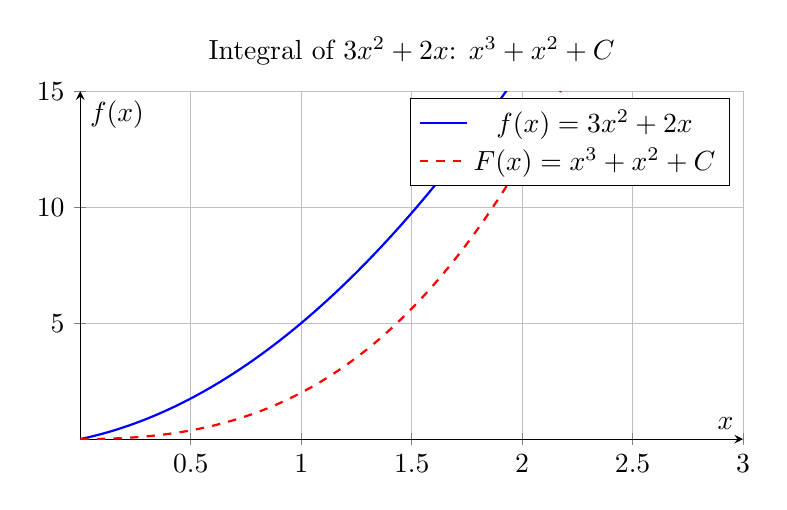
\begin{tikzpicture}
            \begin{axis}[
                axis lines = middle,
                xlabel = $x$,
                ylabel = {$f(x)$},
                ymin=0, ymax=15,
                xmin=0, xmax=3,
                grid = major,
                width=10cm,
                height=6cm,
                domain=0:3,
                samples=100,
                title={Integral of $3x^2 + 2x$: $x^3 + x^2 + C$}
            ]
            \addplot[blue, thick] {3*x^2 + 2*x};
            \addplot[red, thick, dashed, domain=0:3] {x^3 + x^2};
            \legend{$f(x) = 3x^2 + 2x$, $F(x) = x^3 + x^2 + C$}
        \end{axis}
        \end{tikzpicture}
        \captionof{figure}{Graph of $f(x) = 3x^2 + 2x$ (blue) and its antiderivative $F(x) = x^3 + x^2 + C$ (red dashed).}
    \end{center}
\end{enumerate}

\section{Applications of Integrals}
Integrals have many practical applications, especially when you need to calculate totals, such as:
\begin{enumerate}
    \item \textbf{Area Under a Curve:} If you want to calculate the total area under a curve, integrals provide the solution. This is particularly useful in physics and engineering, for example, to find the total distance a car has traveled given its velocity function.

    \textbf{Example:} If the velocity of a car is given by \( f(t) = 2t \), the integral of this function gives the distance traveled:
    \[
    \int 2t \, dt = t^2 + C
    \]
    This means that the distance traveled by the car over time \( t \) is given by \( t^2 + C \).

    \begin{center}
        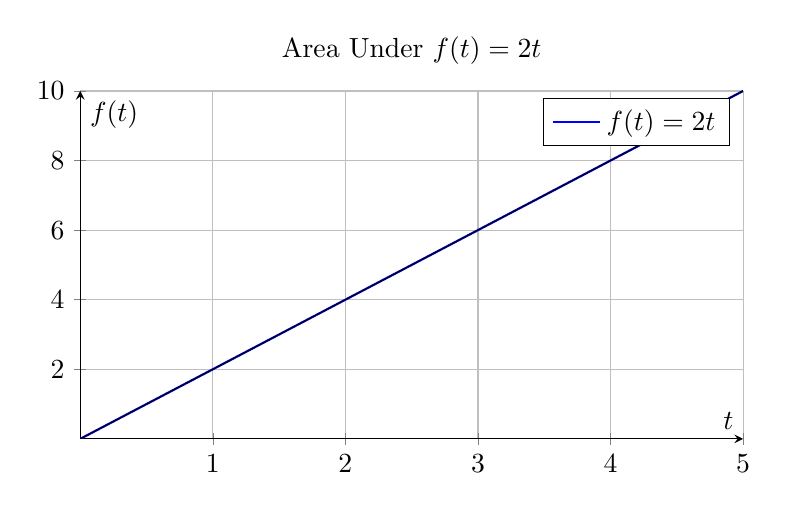
\begin{tikzpicture}
            \begin{axis}[
                axis lines = middle,
                xlabel = $t$,
                ylabel = {$f(t)$},
                ymin=0, ymax=10,
                xmin=0, xmax=5,
                grid = major,
                width=10cm,
                height=6cm,
                domain=0:5,
                samples=100,
                title={Area Under $f(t) = 2t$}
            ]
            \addplot[blue, thick] {2*x};
            \addplot[fill=blue, fill opacity=0.2] coordinates {(0,0) (1,2) (2,4) (3,6) (4,8) (5,10)};
            \legend{$f(t) = 2t$}
        \end{axis}
        \end{tikzpicture}
        \captionof{figure}{The area under the curve $f(t) = 2t$ from $t = 0$ to $t = 5$ represents the total distance traveled.}
    \end{center}

    \item \textbf{Accumulating Quantities:} When you know the rate at which something is changing, you can use integrals to find the total amount accumulated over time. For example, if you know the rate at which water flows into a tank, you can use an integral to find the total volume of water accumulated over a given time period.

    \begin{center}
        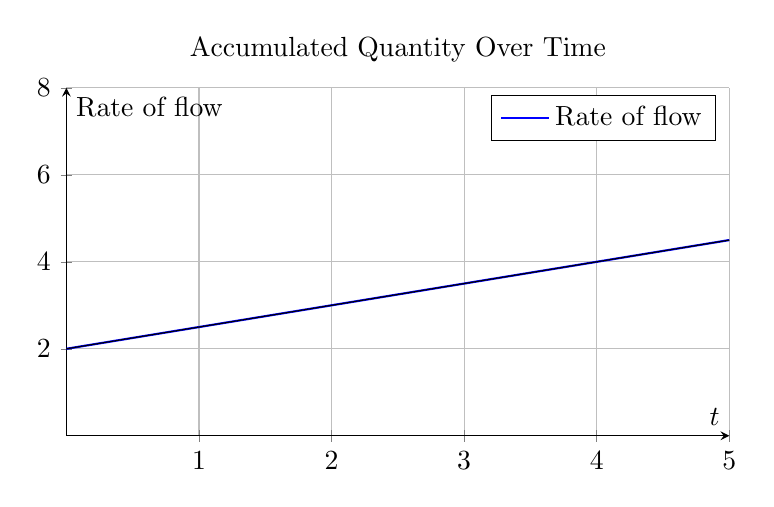
\begin{tikzpicture}
            \begin{axis}[
                axis lines = middle,
                xlabel = $t$,
                ylabel = {Rate of flow},
                ymin=0, ymax=8,
                xmin=0, xmax=5,
                grid = major,
                width=10cm,
                height=6cm,
                domain=0:5,
                samples=100,
                title={Accumulated Quantity Over Time}
            ]
            \addplot[blue, thick] {2 + 0.5*x};
            \addplot[fill=blue, fill opacity=0.2] coordinates {(0,2) (1,2.5) (2,3) (3,3.5) (4,4) (5,4.5)};
            \legend{Rate of flow}
        \end{axis}
        \end{tikzpicture}
        \captionof{figure}{The area under the rate of flow curve represents the total volume of water accumulated in the tank over time.}
    \end{center}

    \item \textbf{Economics and Finance:} In economics, integrals are used to calculate quantities such as consumer and producer surplus by finding the area under demand or supply curves. These integrals represent the total benefit or cost over a range of prices or quantities.

    \begin{center}
        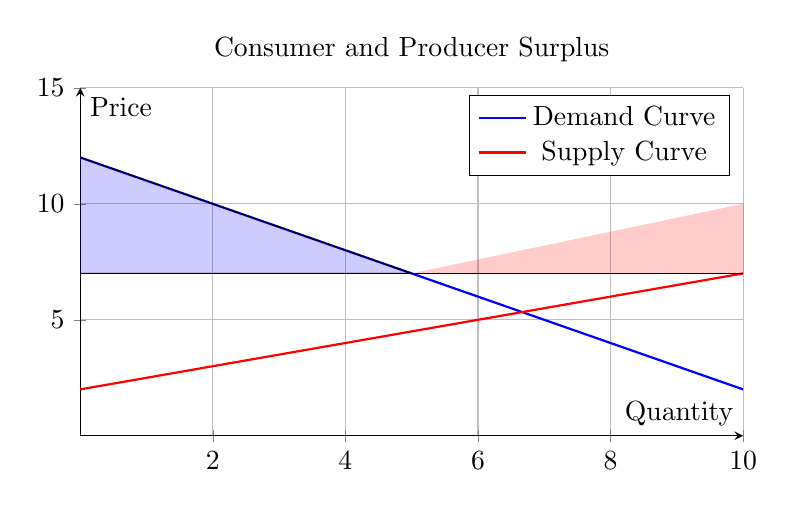
\begin{tikzpicture}
            \begin{axis}[
                axis lines = middle,
                xlabel = Quantity,
                ylabel = {Price},
                ymin=0, ymax=15,
                xmin=0, xmax=10,
                grid = major,
                width=10cm,
                height=6cm,
                domain=0:10,
                samples=100,
                title={Consumer and Producer Surplus}
            ]
            \addplot[blue, thick] {-x + 12};
            \addplot[red, thick] {0.5*x + 2};
            \addplot[fill=blue, fill opacity=0.2] coordinates {(0,12) (5,7) (0,7)};
            \addplot[fill=red, fill opacity=0.2] coordinates {(5,7) (10,7) (10,10)};
            \legend{Demand Curve, Supply Curve}
        \end{axis}
        \end{tikzpicture}
        \captionof{figure}{The area between the demand and supply curves represents the consumer and producer surplus.}
    \end{center}
\end{enumerate}



\section{Fundamental Theorem of Calculus}
The Fundamental Theorem of Calculus links derivatives and integrals. It states that:
\begin{enumerate}
    \item The derivative of the integral of a function is the function itself.
    \item The integral of the derivative of a function gives you the accumulated value of the function.
\end{enumerate}
In simple terms, derivatives and integrals are two sides of the same coin—one describes how something is changing, while the other describes how much has accumulated.

\section{Practice Makes Perfect: Let’s Try Some Exercises!}
\subsection{Derivatives}
\begin{enumerate}
    \item Find the derivative of \( f(x) = 4x^3 \).
    \item Find the derivative of \( f(x) = x^2 + 3x + 2 \).
\end{enumerate}

\subsection{Integrals}
\begin{enumerate}
    \item Find the integral of \( f(x) = x^2 \).
    \item Find the integral of \( f(x) = 3x + 5 \).
\end{enumerate}

\subsection{Applications}
\begin{enumerate}
    \item A car’s position is given by \( f(t) = t^2 + 2t \). Find the car’s velocity by taking the derivative.
    \item Find the area under the curve \( f(x) = 2x \) between \( x = 0 \) and \( x = 3 \).
\end{enumerate}

\section{Real-Life Applications of Calculus}
\begin{itemize}
    \item \textbf{Physics:} Calculus helps in understanding motion, forces, and energy. Derivatives are used to find velocities and accelerations, while integrals calculate distances and areas under curves.
    \item \textbf{Engineering:} Engineers use calculus to model systems that involve changes, such as heat flow, structural loads, and electrical circuits.
    \item \textbf{Medicine:} In pharmacokinetics, integrals help calculate the total amount of a drug in the bloodstream over time, while derivatives describe how quickly the drug is absorbed or eliminated.
\end{itemize}

\section{Chapter Summary}
\begin{itemize}
    \item Derivatives measure the rate of change of a function. They tell us how fast something is changing at a particular moment.
    \item Integrals measure accumulation. They help us calculate the total amount of something, such as the area under a curve.
    \item The Fundamental Theorem of Calculus connects derivatives and integrals, showing that they are inverse operations.
    \item Calculus has many real-world applications, from physics and engineering to economics and medicine.
\end{itemize}

\section{Challenge Questions}

\begin{enumerate}
    \item \textbf{Challenge Question 1:} A car’s acceleration is given by \( a(t) = 4t \), where \( t \) is time in seconds. Find the car’s velocity at \( t = 5 \) seconds if its initial velocity at \( t = 0 \) is \( 2 \, \text{m/s} \).
    
    \begin{center}
        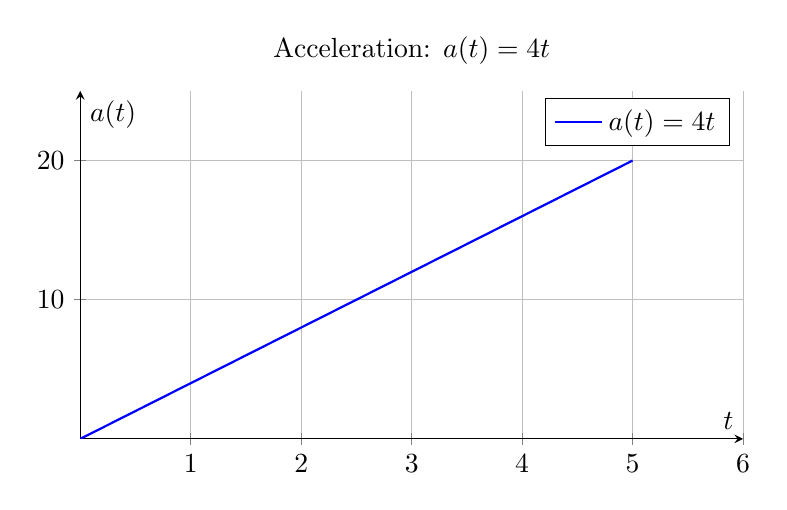
\begin{tikzpicture}
            \begin{axis}[
                axis lines = middle,
                xlabel = $t$,
                ylabel = {$a(t)$},
                ymin=0, ymax=25,
                xmin=0, xmax=6,
                grid = major,
                width=10cm,
                height=6cm,
                domain=0:5,
                samples=100,
                title={Acceleration: $a(t) = 4t$}
            ]
            \addplot[blue, thick] {4*x};
            \legend{$a(t) = 4t$}
        \end{axis}
        \end{tikzpicture}
    \end{center}

    \item \textbf{Challenge Question 2:} The rate of water flow into a tank is given by \( f(t) = 5 \sin(t) \) liters per second. Find the total volume of water in the tank after \( t = \pi \) seconds.
    
    \begin{center}
        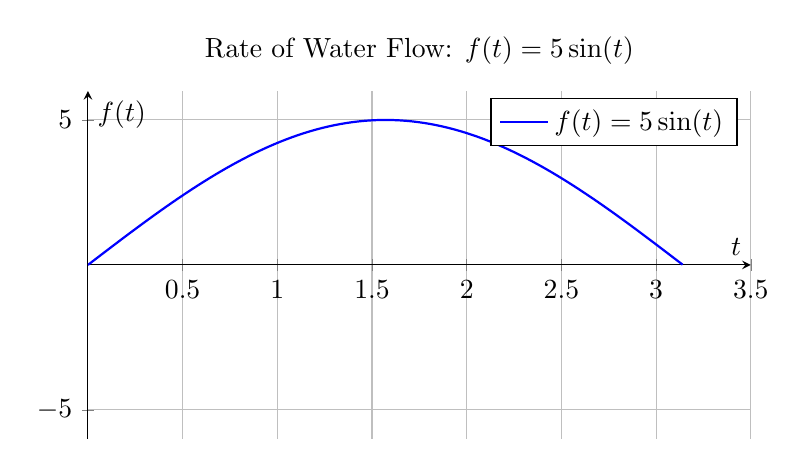
\begin{tikzpicture}
            \begin{axis}[
                axis lines = middle,
                xlabel = $t$,
                ylabel = {$f(t)$},
                ymin=-6, ymax=6,
                xmin=0, xmax=3.5,
                grid = major,
                width=10cm,
                height=6cm,
                domain=0:3.14,
                samples=100,
                title={Rate of Water Flow: $f(t) = 5 \sin(t)$}
            ]
            \addplot[blue, thick] {5 * sin(deg(x))};
            \legend{$f(t) = 5 \sin(t)$}
        \end{axis}
        \end{tikzpicture}
    \end{center}

    \item \textbf{Challenge Question 3:} The demand for a product is given by \( D(q) = 20 - q \) where \( q \) is the quantity demanded. Find the consumer surplus when the market price is \$10.
    
    \begin{center}
        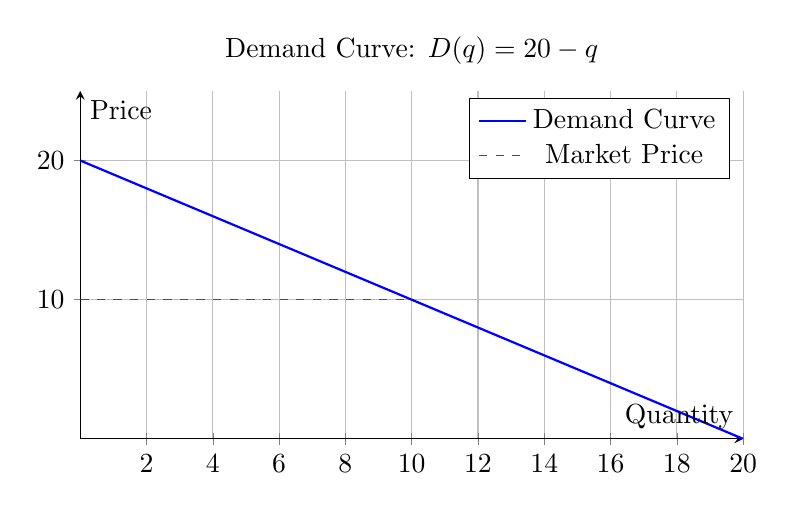
\begin{tikzpicture}
            \begin{axis}[
                axis lines = middle,
                xlabel = Quantity,
                ylabel = {Price},
                ymin=0, ymax=25,
                xmin=0, xmax=20,
                grid = major,
                width=10cm,
                height=6cm,
                domain=0:20,
                samples=100,
                title={Demand Curve: $D(q) = 20 - q$}
            ]
            \addplot[blue, thick] {20 - x};
            \addplot[red, dashed] coordinates {(0,10) (10,10)};
            \legend{Demand Curve, Market Price}
        \end{axis}
        \end{tikzpicture}
    \end{center}

    \item \textbf{Challenge Question 4:} Find the total area enclosed by the curve \( f(x) = x^3 - 3x \) and the x-axis between \( x = -2 \) and \( x = 2 \).
    
    \begin{center}
        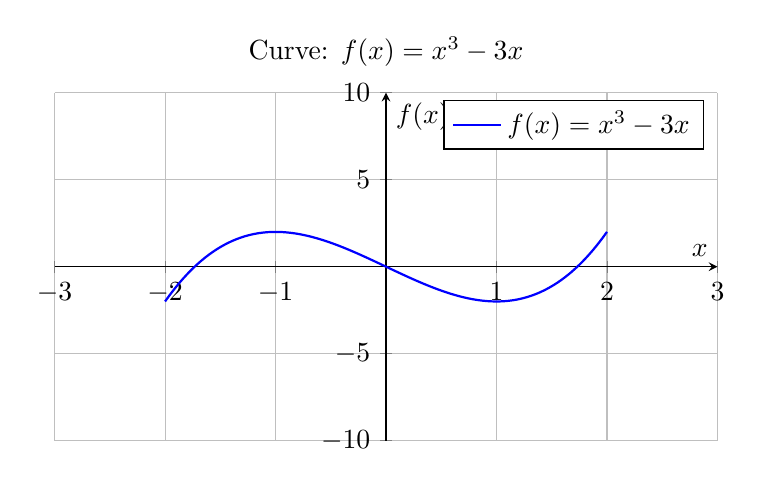
\begin{tikzpicture}
            \begin{axis}[
                axis lines = middle,
                xlabel = $x$,
                ylabel = {$f(x)$},
                ymin=-10, ymax=10,
                xmin=-3, xmax=3,
                grid = major,
                width=10cm,
                height=6cm,
                domain=-2:2,
                samples=100,
                title={Curve: $f(x) = x^3 - 3x$}
            ]
            \addplot[blue, thick] {x^3 - 3*x};
            \legend{$f(x) = x^3 - 3x$}
        \end{axis}
        \end{tikzpicture}
    \end{center}

    \item \textbf{Challenge Question 5:} A particle moves along a line such that its velocity is given by \( v(t) = 4e^{-0.5t} \). Find the total distance traveled by the particle from \( t = 0 \) to \( t = 6 \).
    
    \begin{center}
        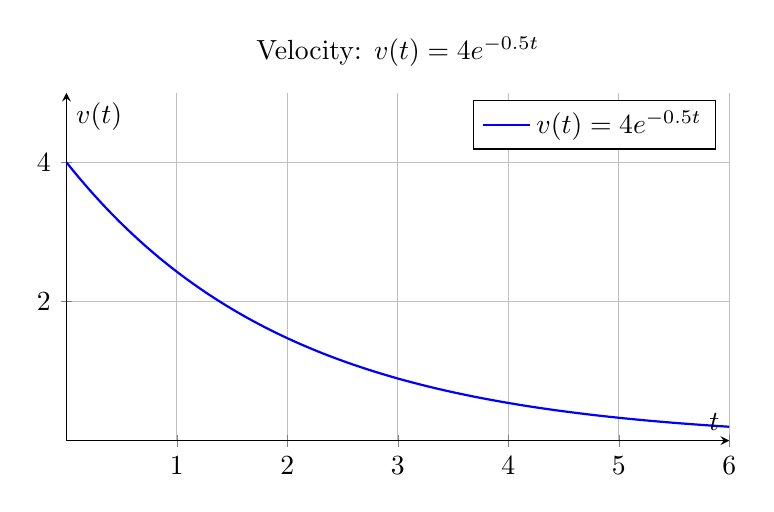
\begin{tikzpicture}
            \begin{axis}[
                axis lines = middle,
                xlabel = $t$,
                ylabel = {$v(t)$},
                ymin=0, ymax=5,
                xmin=0, xmax=6,
                grid = major,
                width=10cm,
                height=6cm,
                domain=0:6,
                samples=100,
                title={Velocity: $v(t) = 4e^{-0.5t}$}
            ]
            \addplot[blue, thick] {4 * exp(-0.5*x)};
            \legend{$v(t) = 4e^{-0.5t}$}
        \end{axis}
        \end{tikzpicture}
    \end{center}

    \item \textbf{Challenge Question 6:} Given the marginal cost function \( C'(x) = 3x^2 + 2x + 1 \), find the total cost of producing 5 units if the fixed cost is 10.
    
    \begin{center}
        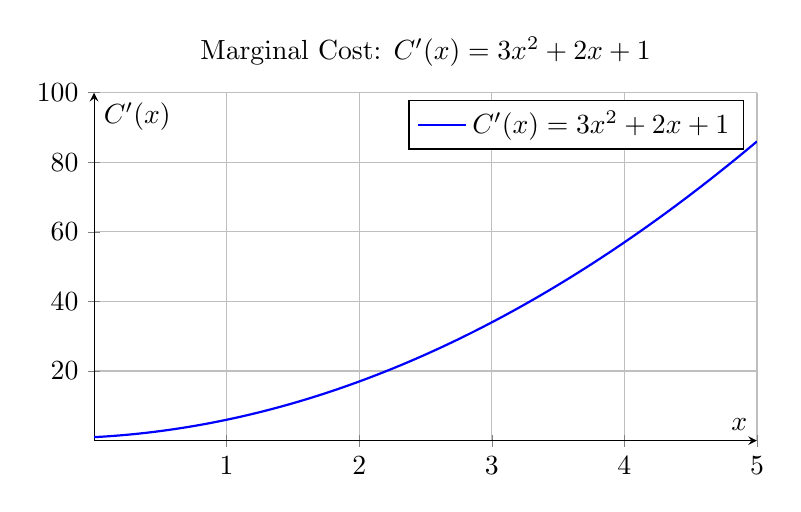
\begin{tikzpicture}
            \begin{axis}[
                axis lines = middle,
                xlabel = $x$,
                ylabel = {$C'(x)$},
                ymin=0, ymax=100,
                xmin=0, xmax=5,
                grid = major,
                width=10cm,
                height=6cm,
                domain=0:5,
                samples=100,
                title={Marginal Cost: $C'(x) = 3x^2 + 2x + 1$}
            ]
            \addplot[blue, thick] {3*x^2 + 2*x + 1};
            \legend{$C'(x) = 3x^2 + 2x + 1$}
        \end{axis}
        \end{tikzpicture}
    \end{center}

    \item \textbf{Challenge Question 7:} A bacteria population grows at a rate given by \( r(t) = 100e^{0.2t} \). Find the total population growth from \( t = 0 \) to \( t = 5 \).
    
    \begin{center}
        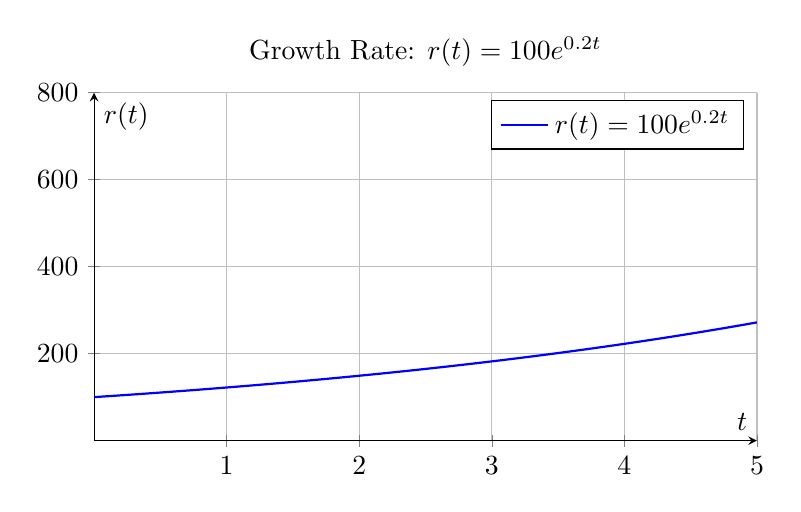
\begin{tikzpicture}
            \begin{axis}[
                axis lines = middle,
                xlabel = $t$,
                ylabel = {$r(t)$},
                ymin=0, ymax=800,
                xmin=0, xmax=5,
                grid = major,
                width=10cm,
                height=6cm,
                domain=0:5,
                samples=100,
                title={Growth Rate: $r(t) = 100e^{0.2t}$}
            ]
            \addplot[blue, thick] {100 * exp(0.2*x)};
            \legend{$r(t) = 100e^{0.2t}$}
        \end{axis}
        \end{tikzpicture}
    \end{center}

    \item \textbf{Challenge Question 8:} The temperature in a room changes over time according to \( T(t) = 20 + 5 \sin(0.5t) \). Find the average temperature in the room over \( t = 0 \) to \( t = 4\pi \).
    
    \begin{center}
        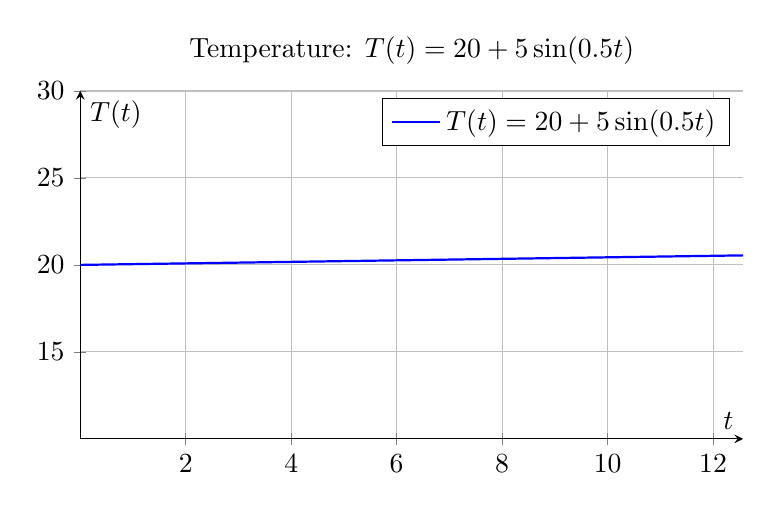
\begin{tikzpicture}
            \begin{axis}[
                axis lines = middle,
                xlabel = $t$,
                ylabel = {$T(t)$},
                ymin=10, ymax=30,
                xmin=0, xmax=12.57,
                grid = major,
                width=10cm,
                height=6cm,
                domain=0:12.57,
                samples=100,
                title={Temperature: $T(t) = 20 + 5 \sin(0.5t)$}
            ]
            \addplot[blue, thick] {20 + 5 * sin(0.5 * x)};
            \legend{$T(t) = 20 + 5 \sin(0.5t)$}
        \end{axis}
        \end{tikzpicture}
    \end{center}

    \item \textbf{Challenge Question 9:} An object’s velocity is given by \( v(t) = 3t^2 - 12t + 9 \). Find the time \( t \) at which the object comes to rest within the interval \( t = 0 \) to \( t = 5 \).
    
    \begin{center}
        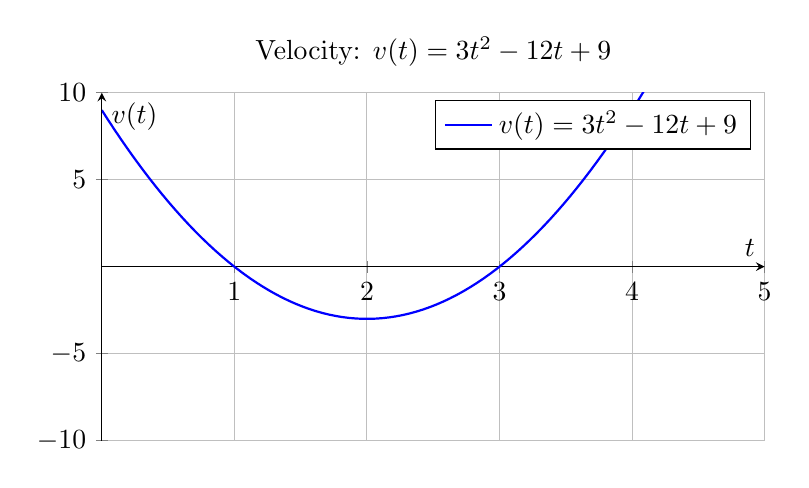
\begin{tikzpicture}
            \begin{axis}[
                axis lines = middle,
                xlabel = $t$,
                ylabel = {$v(t)$},
                ymin=-10, ymax=10,
                xmin=0, xmax=5,
                grid = major,
                width=10cm,
                height=6cm,
                domain=0:5,
                samples=100,
                title={Velocity: $v(t) = 3t^2 - 12t + 9$}
            ]
            \addplot[blue, thick] {3*x^2 - 12*x + 9};
            \legend{$v(t) = 3t^2 - 12t + 9$}
        \end{axis}
        \end{tikzpicture}
    \end{center}

    \item \textbf{Challenge Question 10:} Find the area between the curve \( f(x) = x^2 - 4 \) and the x-axis from \( x = -2 \) to \( x = 2 \).
    
    \begin{center}
        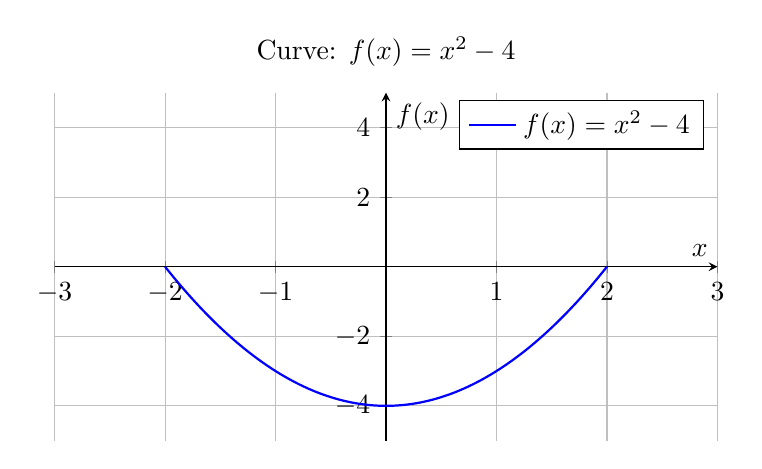
\begin{tikzpicture}
            \begin{axis}[
                axis lines = middle,
                xlabel = $x$,
                ylabel = {$f(x)$},
                ymin=-5, ymax=5,
                xmin=-3, xmax=3,
                grid = major,
                width=10cm,
                height=6cm,
                domain=-2:2,
                samples=100,
                title={Curve: $f(x) = x^2 - 4$}
            ]
            \addplot[blue, thick] {x^2 - 4};
            \legend{$f(x) = x^2 - 4$}
        \end{axis}
        \end{tikzpicture}
    \end{center}
\end{enumerate}
